\begin{figure}[!htbp]\centering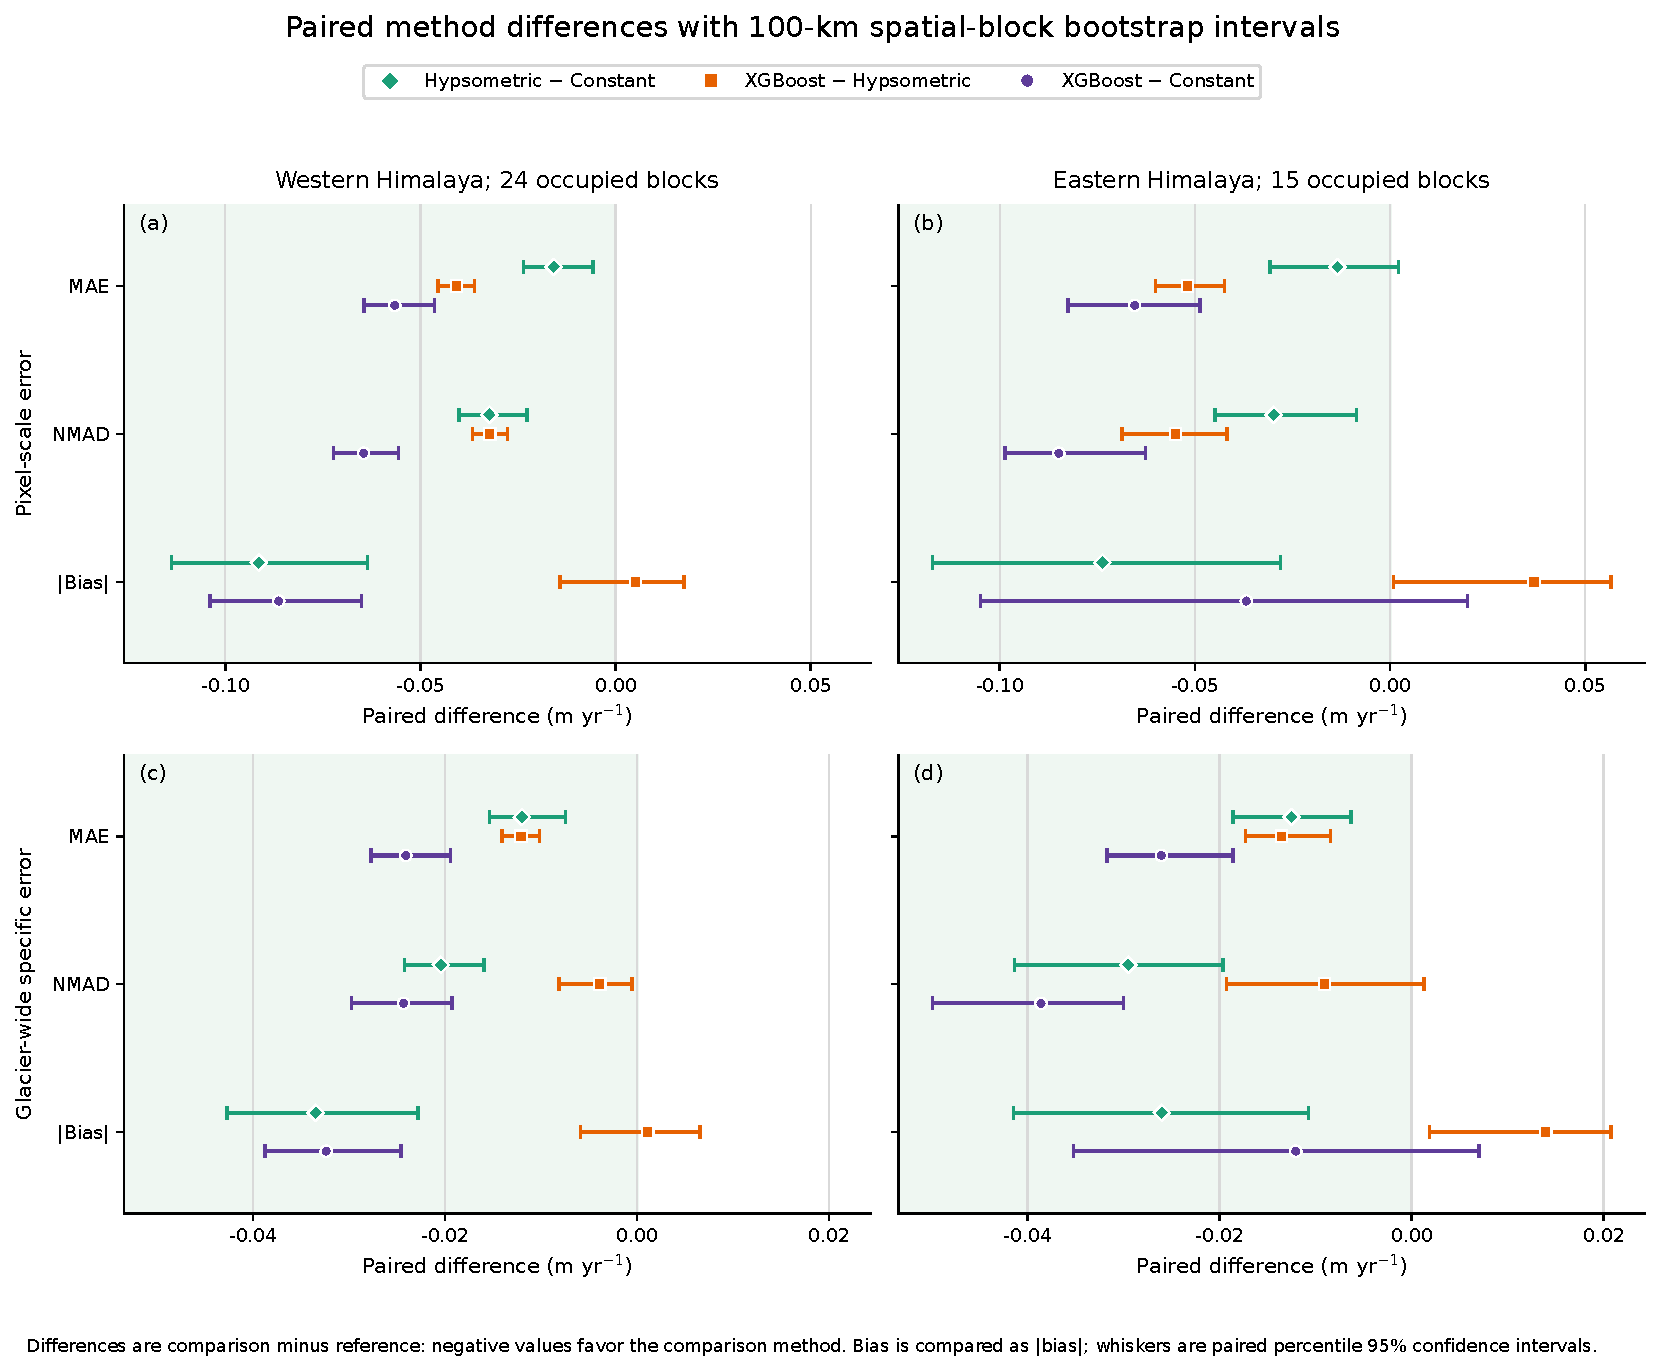
\includegraphics[width=\textwidth,height=.62\textheight,keepaspectratio]{fig04_bootstrap_contrasts.pdf}\caption{Paired method contrasts for pixel errors (a,b) and glacier-wide specific errors (c,d) in the Western (left) and Eastern (right) Himalaya. Symbols show comparison-minus-baseline differences in MAE, NMAD, and absolute bias for the three method pairs identified in the legend. Negative values indicate a lower error metric for the comparison method. Bias contrasts subtract the magnitudes of population mean signed errors. Bars show 95\% percentile intervals from 2,000 paired spatial-block bootstrap draws using 100 km blocks, with all realizations of each glacier retained together. The evaluated test population excludes RGI60-14.17287.}\label{fig:bootstrap}\end{figure}

